% Demo and documentation for qtree.sty, the front end to the 
% Qobitree tree-drawing package

% (LaTeX)

\documentclass[11pt,a4paper]{ltxdoc}

\usepackage{tikz}
\usepackage{tikz-qtree}
\usetikzlibrary{positioning}
\newcommand{\MonetaryLevel}{Monetary level}
\newcommand{\RealLevel}{Real level}
\newcommand{\Firms}{Firms}
\newcommand{\Households}{Households}
\newcommand{\Banks}{Banks}
\newcommand{\Commodities}{Commodities}
\newcommand{\LaborPower}{Labor power}
\newcommand{\Wages}{Wages}
\newcommand{\Consumption}{Consumption}
\newcommand{\Credits}{Credits}
\newcommand{\Withdrawals}{Withdrawals}
\newcommand{\Deposits}{Deposits}
\newcommand{\Repayments}{Repayments}

\newcommand{\yslant}{0.5}
\newcommand{\xslant}{-0.6}
\begin{document}
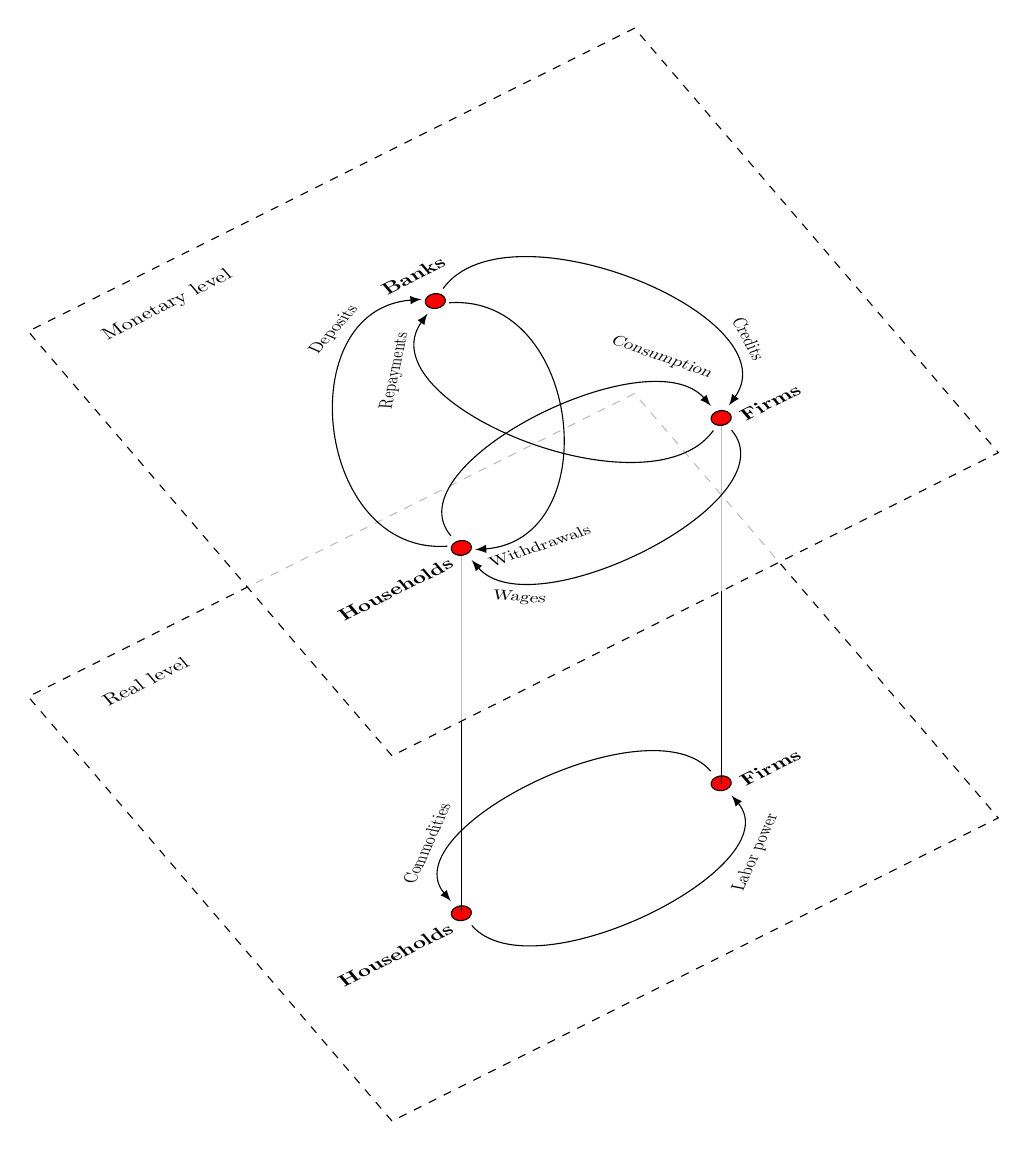
\begin{tikzpicture}[scale=1.1,every node/.style={minimum size=1cm},on grid]

	% Real level
	\begin{scope}[
		yshift=-120,
		every node/.append style={yslant=\yslant,xslant=\xslant},
		yslant=\yslant,xslant=\xslant
	] 
		% The frame:
		\draw[black, dashed, thin] (0,0) rectangle (7,7); 
		% Agents:
		\draw[fill=red]  
			(5,2) circle (.1) % Firms
			(2,2) circle (.1); % Households
		% Flows:
		\draw[-latex,thin] 
			(2,1.8) to[out=-90,in=-90] (5,1.8); % Labour Powers
		\draw[-latex,thin]
			(5,2.2) to[out=90,in=90] (2,2.2); % Wages
		 % Labels:
		\fill[black]
			(0.5,6.5) node[right, scale=.7] {\RealLevel}	
			(5.1,1.9) node[right,scale=.7]{\textbf{\Firms}}
			(1.9,1.9) node[left,scale=.7]{\textbf{\Households}}
			(2.2,3) node [scale=.6, rotate=40] {\Commodities} 
			(4.8,1) node [scale=.6, rotate=40] {\LaborPower};	
	\end{scope}
	
	% 2 vertical lines for linking agents on the 2 levels
	\draw[ultra thin](3.8,4) to (3.8,-0.32);
	\draw[ultra thin](.8,2.4) to (.8,-1.8);
	
	% Monetary level
	\begin{scope}[
		yshift=0,
		every node/.append style={yslant=\yslant,xslant=\xslant},
		yslant=\yslant,xslant=\xslant
	]
		% The frame:
		\fill[white,fill opacity=.75] (0,0) rectangle (7,7); % Opacity
		\draw[black, dashed, thin] (0,0) rectangle (7,7); 
		 % Agents:
		\draw [fill=red]
			(5,2) circle (.1) % Firms
			(2,2) circle (.1) % Households
			(3.5,5) circle (.1); % Banks
		 % Monetary Flows:
		\draw[-latex, thin]
			(3.65,5.1) to[out=30,in=30] (5.15,2.1); % Credits
		\draw[-latex, thin]
			(5,1.8) to[out=-90,in=-90] (2,1.8); % Wages
		\draw[-latex, thin]
			(1.9,2.1) to[out=150,in=150] (3.4,5.1);  % Deposits
		\draw[-latex, thin]
			(3.6,4.9) to[out=-30,in=-30] (2.1,1.9); % Withdrawals
		\draw[-latex, thin]
			(2,2.2) to[out=90,in=90] (5,2.2); % Consumption
		\draw[-latex, thin]
			(4.85,1.9) to[out=210,in=210] (3.35,4.9) ; % Repayments
		 % Labels:
		\fill[black]
			(0.5,6.5) node[right, scale=.7] {\MonetaryLevel}
			(5.1,1.9) node[right,scale=.7]{\textbf {\Firms}}
			(1.9,1.9) node[left,scale=.7]{\textbf {\Households}}
			(3.5,5.1) node[above,scale=.7]{\textbf {\Banks}}
			(5.5,2.8) node [above, scale=.6, rotate=-100] {\Credits}
			(2.6,1.3) node [above, scale=.6, rotate=-10] {\Withdrawals}
			(2.9,4.25) node [above, scale=.6, rotate=50] {\Repayments}
			(2.6,5) node [above, scale=.6, rotate=25] {\Deposits}
			(4.7,2.9) node [above, scale=.6, rotate=-60] {\Consumption}
			(2.3,1.3) node [below, scale=.6, rotate=-40] {\Wages}; 
	\end{scope} 
\end{tikzpicture}
